\documentclass{article}
\usepackage{amsmath}
\usepackage{tikz}
\usetikzlibrary{arrows.meta}

\begin{document}

\begin{center}
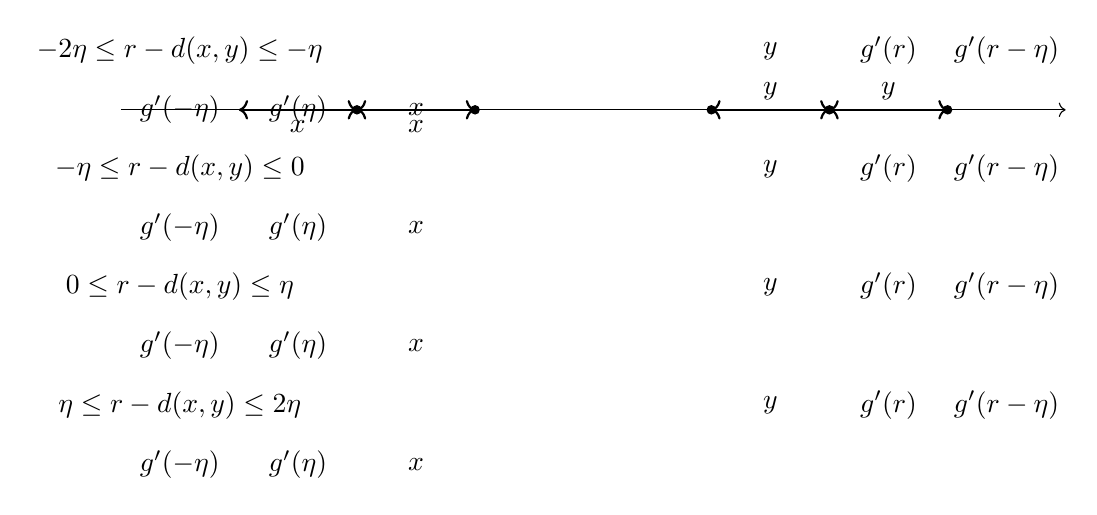
\begin{tikzpicture}[scale=1.5]
    % Draw the horizontal axis
    \draw[->] (-4,0) -- (4,0);
    
    % Define points
    \coordinate (A) at (-3,0);
    \coordinate (B) at (-2,0);
    \coordinate (C) at (-1,0);
    \coordinate (D) at (1,0);
    \coordinate (E) at (2,0);
    \coordinate (F) at (3,0);
    
    % Draw arrows
    \draw[<->,thick] (A) -- node[below] {$x$} (B);
    \draw[<->,thick] (B) -- node[below] {$x$} (C);
    \draw[<->,thick] (D) -- node[above] {$y$} (E);
    \draw[<->,thick] (E) -- node[above] {$y$} (F);
    
    % Draw circles
    \filldraw (B) circle (1pt);
    \filldraw (C) circle (1pt);
    \filldraw (D) circle (1pt);
    \filldraw (E) circle (1pt);
    \filldraw (F) circle (1pt);
    
    % Draw labels
    \node at (-3.5,0.5) {$-2\eta \leq r - d(x,y) \leq -\eta$};
    \node at (-3.5,0) {$g'(-\eta)$};
    \node at (-2.5,0) {$g'(\eta)$};
    \node at (-1.5,0) {$x$};
    
    \node at (-3.5,-0.5) {$-\eta \leq r - d(x,y) \leq 0$};
    \node at (-3.5,-1) {$g'(-\eta)$};
    \node at (-2.5,-1) {$g'(\eta)$};
    \node at (-1.5,-1) {$x$};
    
    \node at (-3.5,-1.5) {$0 \leq r - d(x,y) \leq \eta$};
    \node at (-3.5,-2) {$g'(-\eta)$};
    \node at (-2.5,-2) {$g'(\eta)$};
    \node at (-1.5,-2) {$x$};
    
    \node at (-3.5,-2.5) {$\eta \leq r - d(x,y) \leq 2\eta$};
    \node at (-3.5,-3) {$g'(-\eta)$};
    \node at (-2.5,-3) {$g'(\eta)$};
    \node at (-1.5,-3) {$x$};
    
    \node at (3.5,0.5) {$g'(r-\eta)$};
    \node at (2.5,0.5) {$g'(r)$};
    \node at (1.5,0.5) {$y$};
    
    \node at (3.5,-0.5) {$g'(r-\eta)$};
    \node at (2.5,-0.5) {$g'(r)$};
    \node at (1.5,-0.5) {$y$};
    
    \node at (3.5,-1.5) {$g'(r-\eta)$};
    \node at (2.5,-1.5) {$g'(r)$};
    \node at (1.5,-1.5) {$y$};
    
    \node at (3.5,-2.5) {$g'(r-\eta)$};
    \node at (2.5,-2.5) {$g'(r)$};
    \node at (1.5,-2.5) {$y$};
\end{tikzpicture}
\end{center}

\caption{The intervals satisfying \( h_{x,\lambda,\eta}^+(\phi_s g') h_{y,\lambda,\eta}^-( \phi_{r+s}g') \neq 0 \)}

\end{document}